\documentclass[a4paper, 12pt, oneside, titlepage, BCOR=1mm, DIV=12]{article}
\usepackage[a4paper,top=2cm,bottom=2cm,left=1cm,right=1cm]{geometry}

\usepackage[utf8]{inputenc}
\usepackage[english,ukrainian]{babel}
\usepackage[document]{ragged2e}
\usepackage{fancyhdr}
\usepackage{mathtext}
\usepackage{scrextend}
\usepackage{eqnarray,amsmath,amssymb}
\usepackage{color}
\usepackage{setspace}
\usepackage{graphicx}
\usepackage{hyperref}

\newcommand{\Lim}[1]{\raisebox{0.5ex}{{$\displaystyle \lim_{#1}\;$}}}


% checkboxes! щоб перевіряти чи правильно

\renewcommand{\d}[1]{
  \hspace{2pt}\text{d}\hspace{1pt}{#1}
}

\newcommand{\dx}{\hspace{2pt}\text{ERRROR}}
\newcommand{\dt}{\hspace{2pt}\text{ERRROR}}
\newcommand{\du}{\hspace{2pt}\text{ERRROR}}
\newcommand{\dv}{\hspace{2pt}\text{ERRROR}}
\newcommand{\dw}{\hspace{2pt}\text{ERRROR}}

\definecolor{orange}{RGB}{255,65,0}
\definecolor{red}{RGB}{255,0,0}
\definecolor{gray}{RGB}{190,190,190}
\definecolor{green}{RGB}{0,128,0}

\newcommand{\task}[2]{
  % pre print option
  % \framebox[4cm]{ \par $\square$ {\color{#1}#2} }

  % e-paper check boxes
  \framebox[4cm]{ \par \hspace*{-.3cm}{\CheckBox[width=10pt,height=10pt,bordercolor=0 0 0,name=#2]{\null}} {\color{#1}#2}} }
}
\newcommand{\descr}[2][.5]{
    %\begin{addmargin}[3.5cm]{0cm}
    {\color{white}\fbox{
        \parbox[c][#1cm][l]{.7\textwidth}{
          {\color{black}#2}
        }
      }
    }

    %\end{addmargin}
}





\begin{document}


  % \begin{center}
  %   \Large{\cyr{\textbf{Математичний Аналіз - Практичний варіант}}} \\
  % \end{center}

  % Границі та похідні
  %
  \pagenumbering{gobble}
\clearpage
\vspace*{\fill}
\begin{center}

  \begin{minipage}{1\textwidth}
    \begin{center}\LARGE{\cyr{\textbf{Розрахункова Робота}}}\end{center}
    \begin{center}\large{\cyr{\textbf{з дискретної математики}}}\end{center}

    \begin{center}
      \normalsize{\cyr{\textbf{студента групи ICзп 71}}} \\
      \normalsize{\cyr{\textbf{Бутузова О. В.}}}
    \end{center}

    \begin{center}
      \normalsize{\cyr{\textbf{Варіант №4}}}
    \end{center}


  \end{minipage}

\end{center}
\vfill % equivalent to \vspace{\fill}
\clearpage

  Загальне
  \begin{itemize}
\item В данній розрахунковій роботі відсутній розв'язок завдання #7б (07.02)
\end{itemize}

  Розрахункова робота - 1
  \begin{itemize}
\item В данній розрахунковій роботі відсутній розв'язок завдання #7б (07.02)
\end{itemize}

  \pagebreak

  {\task{green}{В4 - РР1 - 01.01}} \begin{center}\large{\cyr{\textbf{1.1 Довести тотожність аксіоматично}}}\end{center}

\begin{displaymath}
  A\cup((B\bigtriangleup(B\bigtriangleup{A})) \setminus B)=A
\end{displaymath}

Спростимо ліву частину завдиння поступово спрощуючи формули за допомогою основних та похідних законів алгебри множин (для кращого розуміння ходу процесу кожна дія обмежена одною-двома операціями):

$$
A\cup((B\bigtriangleup(B\bigtriangleup{A})) \setminus B) = A
$$

\begin{displaymath}


  \text{ Операції $\setminus$ та $\bigtriangleup$ розкривати за формулами: }\\
  A\setminus{B}=A\cap{B}\compl \\qquad A\bigtriangleup{B} = (A\cap{B\compl})\cup{(B\cap{A\compl} )}

\end{displaymath}

\begin{center}\normalsize{\cyr{\textbf{Розкриття}}}\end{center}
\begin{array}{l}

  A = A\cup{((B\bigtriangleup(B\bigtriangleup{A})) \setminus B)}   \\
  A = A\cup{((B\bigtriangleup(  ( ( A\compl \cap{B} )  \cup{ ( A \cap{B\compl} )} )  )) \setminus B)}   \\
  A = A\cup{(( (  ( ( A\compl \cap{B} )  \cup{ ( A \cap{B\compl} )} ) \compl \cap{B} )  \cup{ (  ( ( A\compl \cap{B} )  \cup{ ( A \cap{B\compl} )} )  \cap{B\compl} )} )  \setminus B)}  \\

  A = A\cup{((((( A\compl \cap{B} )  \cup{ ( A \cap{B\compl} )} ) \compl \cap{B} )  \cup{ (  ( ( A\compl \cap{B} )  \cup{ ( A \cap{B\compl} )} )  \cap{B\compl} )} )  \cap{B\compl} )}   \\

\end{array}


\begin{center}\normalsize{\cyr{\textbf{Доведення}}}\end{center}
$$
\begin{array}{r|l}
  \text{Закони} & \text{Тотожності} \\
  \hline \\
  1      & A \cup ( B\compl \cap ( ( B \cap ( ( A\compl \cap{B}) \cup ( A \cap B\compl ) )\compl ) \cup ( {B\compl} \cap ( ( A\compl\cap{B}) \cup (A \cap B\compl)) )) ) \\
  10,11,1  & A \cup ( B\compl \cap ( ( B \cap  ( ( A\compl \cup B ) \cap ( A \cup B\compl ) ) ) \cup ( B\compl \cap ( ( A\compl \cap B ) \cup ( A \cap B\compl ) ) ) ) ) \\
  2      & A \cup ( B\compl \cap ( ( ( B \cap ( A\compl \cup  B ) ) \cap ( B \cap (  A \cup B\compl ) ) ) \cup ( (B\compl \cap ( A\compl \cap  B ) ) \cap ( B\compl \cap ( A \cap B\compl ) ) ) ) ) \\
  1       & A \cup ( B\compl \cap ( ( ( B \cap (  B \cup A\compl ) ) \cap ( B \cap ( B\compl \cup  A ) ) ) \cup ( (B\compl \cap (  B \cap A\compl ) ) \cap ( B\compl \cap ( B\compl \cap A ) ) ) ) ) \\
  6       & A \cup ( B\compl \cap ( ( ( B \cap ( B \cup A\compl ) ) \cap ( B \cap ( B\compl \cup  A ) ) ) \cup ( (B\compl \cap (  B \cap A\compl ) ) \cap ( B\compl \cap ( B\compl \cap A ) ) ) ) ) \\
  12      & A \cup ( B\compl \cap ( ( B \cap ( B \cap ( B\compl \cup  A ) ) ) \cup ( (B\compl \cap (  B \cap A\compl ) ) \cap ( B\compl \cap ( B\compl \cap A ) ) ) ) ) \\
  8       & A \cup ( B\compl \cap ( ( ( B \cap B )  \cap A  ) \cup ( ( ( B\compl \cap B )  \cap A\compl ) \cap ( ( B\compl \cap B\compl ) \cap A  ) ) ) ) \\
  5,4,7   & A \cup ( B\compl \cap ( ( B \cap A ) \cup ( ( \emptyset \cap A\compl ) \cap (B\compl \cap A ) ) ) \\
  5       & A \cup ( B\compl \cap ( ( B \cap A ) \cup ( \emptyset \cap (B\compl \cap A ) ) ) \\
  3       & A \cup ( B\compl \cap ( ( B \cap A ) \cup \emptyset   ) \\
  8,4       & A \cup ( B\compl \cap ( B \cap A ) ) \\
  5       & A \cup ( \emptyset \cap A   ) \\
  5       & A \cup \emptyset  \\
  3       & A

\end{array}
$$

Тотожність доведено.
 \\ \qquad \\
  {\task{green}{В4 - РР1 - 02.01}} {\descr{Знайти Границю функції}}

$$
  \lim_{n\to\infty} \dfrac{(n+5)^2+(n+4)^2}{(n+3)^3-(n-2)^3} = [ \dfrac{\infty}{\infty}]
$$

$$
  \lim_{n\to\infty} \dfrac{(n+5)^2+(n+4)^2}{(n+3)^3-(n-2)^3} =
  \lim_{n\to\infty} \dfrac{(n+5)(n+5)+(n+4)(n+4)}{(n+3)(n+3)(n+3)-(n-2)(n-2)(n-2)} =
$$
$$
  \lim_{n\to\infty} \dfrac{(n^2+10n+25)+(n^2+8n+16)}{(n^3+9n^2+27n+27)-(n^3-6n^2+12n-8)} =
  \lim_{n\to\infty} \dfrac{2n^2+18n+41}{15n^2+15n+35} =
$$
$$
  \lim_{n\to\infty} \dfrac{2+\dfrac{18}{n}+\dfrac{41}{n^2}}{15+\dfrac{15}{n}+\dfrac{35}{n^2}} =
  % answer!
  \dfrac{2}{15}.
$$

%   розразунки дробної частини (не розкоментовувати) - початок до рохрахунків
%   $$ n^2+n^2+10n+8n+25+16 $$
%   $$(x+3)(x+3)(x+3) = (x+3)(x^2+6x+9) = (x^3+6x^2+3x^2+9x+18x+27) = (x^3+9x^2+27x+27) $$
%   $$(x-2)(x-2)(x-2) = (x-2)(x^2-4x+4) = (x^3-4x^2-2x^2+4x+8x-8)   = (x^3-6x^2+12x-8) $$
%   розразунки дробної частини (не розкоментовувати) - кінець до розрахунків
 \\ \qquad \\
  {\task{green}{В4 - РР1 - 02.02}} \begin{center}\large{\cyr{\textbf{2.2 Обчислити $(R \circ S)^{-1}$ та $(R \circ R^{-1})_{Tr}$}}}\end{center}

$$
R = \{(a_1, b_1), (a_2, b_1), (a_3, b_2)\}, S = \{(b_2, c_1), (b_1, c_2), (b_2, c_3), (b_2, c_4)\}.
$$

$$
R: A \to B,  \quad  R = \left[ \begin{array}{c|ccc}
  & b_1 & b_2 \\
  \hline
  a_1 & 1 & 0 \\
  a_2 & 1 & 0 \\
  a_3 & 0 & 1 \\
  \end{array} \right] \quad
S: B \to C, \quad S=   \left[ \begin{array}{c|cccc}
  & c_1 & c_2 & c_3 & c_4  \\
  \hline
  b_1 & 0 & 1 & 0 & 0 \\
  b_2 & 1 & 0 & 1 & 1 \\
  \end{array} \right]
$$

$$
a) \qquad
R \circ S = \left[ \begin{array}{c|cccc}
  & c_1 & c_2 & c_3 & c_4  \\
  \hline
  a_1 & 0 & 1 & 0 & 0 \\
  a_2 & 0 & 1 & 0 & 0 \\
  a_3 & 1 & 0 & 1 & 1 \\
\end{array} \right]
  (R \circ S)^{-1} \left[ \begin{array}{c|ccc}
 & a_1 & a_2 & a_3 \\
 \hline
 c_1 & 0 & 0 & 1 \\
 c_2 & 1 & 1 & 0 \\
 c_3 & 0 & 0 & 1 \\
 c_4 & 0 & 0 & 1\\
\end{array} \right]
$$

$$
b) \quad R: A \to B,  \quad  R = \left[ \begin{array}{c|ccc}
  & b_1 & b_2 \\
  \hline
  a_1 & 1 & 0 \\
  a_2 & 1 & 0 \\
  a_3 & 0 & 1 \\
  \end{array} \right] \quad \qquad R^{-1}: B \to A,  \quad  R^{-1} = \left[ \begin{array}{c|ccc}
  & a_1 & a_2 & a_3 \\
  \hline
  b_1 & 1 & 1 & 0 \\
  b_2 & 0 & 0 & 1 \\
  \end{array} \right]
$$

$$
(R \circ R^{-1}) = \left[ \begin{array}{l|lll}
     & a_1 & a_2 & a_3 \\
 \hline
 a_1 & 1   & 1   & 0 \\
 a_2 & 1   & 1   & 0 \\
 a_3 & 0   & 0   & 1 \\
\end{array} \right]
$$

$$
\begin{tabular*}{\linewidth}{>{$}r<{$}@{\extracolsep{\fill}}>{$}r<{$}>{$}r<{$}}

    \begin{tikzpicture}[node distance=1cm]
      % nodes
      \node[circle, right] (A1) at (0, 0) {a1};
      \draw[->](0,0) -- (0,2);
      \node[circle, right, single arrow] (A2) at (0, 2) {a2};
      \node[circle, left, single arrow]  (A3) at (3, 1) {a3};
      % % arrows
      \draw[line width=1pt] (0, 0) circle (1pt);
      \draw[line width=1pt] (3, 1) circle (1pt);
      \draw[line width=1pt] (0, 2) circle (1pt);

      \draw[->,line width=.1pt](-.4, 0) circle (.4);
      \draw[->,line width=.1pt](-.4, 2) circle (.4);
      \draw[->,line width=.1pt](3.4, 1) circle (.4);
    \end{tikzpicture}
    &
    \begin{tikzpicture}[node distance=1cm]
      % nodes
      \node[circle, right, single arrow] (A1) at (0, 0) {a1};
      \draw[->](0,0) -- (0,2);
      \node[circle, right, single arrow] (A2) at (0, 2) {a2};
      \draw[->, dashed](0,2) -- (3,1);
      \node[circle, left, single arrow]  (A3) at (3, 1) {a3};
      % % arrows
      \draw[line width=1pt] (0, 0) circle (1pt);
      \draw[line width=1pt] (3, 1) circle (1pt);
      \draw[line width=1pt] (0, 2) circle (1pt);

      \draw[->,line width=.1pt](-.4, 0) circle (.4);
      \draw[->,line width=.1pt](-.4, 2) circle (.4);
      \draw[->,line width=.1pt](3.4, 1) circle (.4);
    \end{tikzpicture}
    &
    \begin{tikzpicture}[node distance=1cm]
      % nodes
      \node[circle, right, single arrow] (A1) at (0, 0) {a1};
      \draw[->](0,0) -- (0,2);
      \node[circle, right, single arrow] (A2) at (0, 2) {a2};
      \draw[->](0,2) -- (3,1);
      \node[circle, left, single arrow]  (A3) at (3, 1) {a3};
      \draw[->, dashed](0,0) -- (3,1);
      % % arrows
      \draw[line width=1pt] (0, 0) circle (1pt);
      \draw[line width=1pt] (3, 1) circle (1pt);
      \draw[line width=1pt] (0, 2) circle (1pt);

      \draw[->,line width=.1pt](-.4, 0) circle (.4);
      \draw[->,line width=.1pt](-.4, 2) circle (.4);
      \draw[->,line width=.1pt](3.4, 1) circle (.4);
    \end{tikzpicture} \\
    R & R \cup R^2 & R \cup R^2 \cup R^3
\end{tabular}
$$

$$ \boxed{R_{Tr} = R \cup R^2 \cup R^3}$
 \\ \qquad \\
  {\task{green}{В4 - РР1 - 02.03}} \begin{center}\large{\cyr{\textbf{2.2 Обчислити фактор-множину $\mathbb{R}^2/_\sim$}}}\end{center}

$$
f(x_1,x_2) = |x_1x_2|, \qquad \alpha = 0;1;4.
$$
 \\ \qquad \\
  {\task{green}{В4 - РР1 - 02.04}} {\descr{Знайти Границю функції}}

  $$ \lim_{x\to0}\dfrac{(1+x)^3-(1+3x)}{x+x^5} = \big[\dfrac{0}{0}\big] $$

$$
  \lim_{x\to0}\dfrac{(1+x)^3-(1+3x)}{x+x^5} =
  \lim_{x\to0}\dfrac{(1+x)(1+x)(1+x)-(1+3x)}{x+x^5} =
$$
$$
  \lim_{x\to0}\dfrac{(1+x)(1+2x+x^2)-(1+3x)}{x+x^5} =
  \lim_{x\to0}\dfrac{(1+2x+x^2+x+2x^2+x^3)-(1+3x)}{x+x^5} =
$$
$$
  \lim_{x\to0}\dfrac{x^3+3x^2}{x^5+x} =
  \lim_{x\to0}\dfrac{x(x^2+3x)}{x(x^4+1)} =
  \lim_{x\to0}\dfrac{x^2+3x}{x^4+1} =  \dfrac{0}{1} = 0
$$
 \\ \qquad \\
  {\task{green}{В4 - РР1 - 02.05}} {\descr{Знайти Границю функції}}

$$ \lim_{x\to{-2}} \dfrac{\sqrt{2-x}-2}{x^2-x-6} = \Big[\dfrac{0}{0}\Big] $$

$$
  \lim_{x\to{-2}} \dfrac{(\sqrt{2-x}-2)}{(x+2)(x-3)} * \dfrac{(\sqrt{2-x}+2)}{(\sqrt{2-x}+2)} =
  \lim_{x\to{-2}} \dfrac{2-x-4}{(x-3)(x+2)(\sqrt{(2-x)}+2)} =
$$
$$
  \lim_{x\to{-2}} \dfrac{-1(x+2)}{(x-3)(x+2)(\sqrt{(2-x)}+2)} =
  \dfrac{-1}{(-2-3)(2+2)} =
  \dfrac{-1}{-5\cdot4} =
  \dfrac{1}{20}.
$$
 \\ \qquad \\
  {\task{green}{В4 - РР1 - 02.06}} {\descr{Обчислити визначений інтеграл}}

$$
  \int^{-1}_{-2} \sqrt{2-7x}\d{x} = \Bigg |
    \begin{array}{l c l l l }
      t = 2-7x           & & \d{x} = (x)'dt  & x_2 = -1 & t_2 = 9 \\
      x = (2-t)/7 & & \d{x} = (2/7 - t/7)' = \dfrac{dt}{7} & x_1 = -2 & t_1 = 16 \\
    \end{array}
  \Bigg | =
  \int^{9}_{16} \sqrt{t} \dfrac{dt}{7}
$$

$$
  \dfrac{1}{7} \cdot \dfrac{t^{1/2+1}}{1/2+1} \Bigg |^9_{16} =
  \dfrac{3\sqrt{t^3}}{14} \Bigg |^9_{16} = \dfrac{3}{14} ( \sqrt{9^3} - \sqrt{16^3} ) =
  \dfrac{3}{14} ( \sqrt{3^{2+3}} - \sqrt{4^{2+3}} ) =
  \dfrac{3}{14} ( 3^3 - 4^3 ) = \dfrac{3(27-64)}{14} = 7 \dfrac{13}{14}.
$$

$$
\boxed{7 \dfrac{13}{14}}
$$
 \\ \qquad \\
  {\task{green}{В4 - РР1 - 02.07}} {\descr{Знайти Границю функції}}

$$
  \lim_{x\to0}(\cos{\pi{x}})^{\dfrac{1}{x\sin{x}}}
= \lim_{x\to0}(1+\cos{\pi{x}}-1)^{\dfrac{1}{x\sin{x}}}
= \lim_{x\to0}\Bigg[ (1+\cos{\pi{x}}-1) \Bigg]^{\dfrac{1}{x\sin{x}}}
$$
$$
= \lim_{x\to0}\Bigg[ (1+\cos{\pi{x}}-1)^{\dfrac{1}{\cos{\pi{x}}-1}} \Bigg]^{\dfrac{1}{x\sin{x}}\dfrac{\cos{\pi{x}}-1}{1}}
= e^{\lim_{x\to0}{\dfrac{\cos{\pi{x}}-1}{x\sin{x}}}}
$$
$$
= e^{\Lim{x\to0}{\dfrac{\cos{\pi{x}}-1}{x\sin{x}}}}
= e^{\Lim{x\to0}{\dfrac{(\cos{\pi{x}}-1)'}{(x\sin{x})'}}}
= e^{\Lim{x\to0}{\dfrac{-\sin{\pi{x}}(\pi{x})'}{(x)'\sin{x}+x(\sin{x})'}}}
$$
$$
= e^{\Lim{x\to0}{\dfrac{-\pi\sin{\pi{x}}}{\sin{x}+x\cos{x}}}}
= e^{\pi \Lim{x\to0}{\dfrac{-\sin{\pi{x}}}{\sin{x}+x\cos{x}}}}
$$

$$
\Bigg |
\begin{array}{lcr}
      \sin{\alpha} \sim \alpha  & , & \alpha \to 0 \\
      \cos{\alpha} \sim 1-\dfrac{\alpha^2}{2} & , & \alpha \to 0
    \end{array}
\Bigg |
$$

$$
= e^{\pi \Lim{x\to0}{ \dfrac{-(\pi{x})'}{(\sin{x}+(x\cos{x}))'}}}
= e^{\pi \Lim{x\to0}{ \dfrac{-\pi}{(\cos{x}+(\cos{x}-x\sin{x}))}}}
= e^{\dfrac{-\pi^2}{\Lim{x\to0}{2\cos{x}-x\sin{x}}}
$$

$$
= e^{\dfrac{-\pi^2}{\Lim{x\to0}{2(1+\dfrac{x^2}{2})-x^2}}}
= e^{\dfrac{-\pi^2}{\Lim{x\to0}{2+\dfrac{2x^2}{2}-x^2}}}
= e^{\dfrac{-\pi^2}{\Lim{x\to0}{2+x^2-x^2}}}
= e^{\dfrac{-\pi^2}{2}}.
$$
 \\ \qquad \\
  {\task{green}{В4 - РР1 - 02.08}} {\descr{Знайти Границю функції}}

$$
  \lim_{x\to{0}} \dfrac{6^x-3^{2x}}{\arctg{4x}-\sin{x}} = \big[ \dfrac{1-1}{0+0}\big] = \big[ \dfrac{0}{0}\big] = \Bigg |
    \begin{array}{rcll}
        \sin{\alpha}   & \sim & \alpha & , \alpha \to 0 \\
        \arctg{\alpha} & \sim & \alpha & , \alpha \to 0 \\
        \alpha^x-1 & \sim & x\ln\alpha & , \alpha \to 0 \\
      \end{array}
  \Bigg | = \lim_{x\to{0}} \dfrac{(6^x-1)-(3^{2x}-1)}{\arctg{4x}-\sin{x}}
$$


$$
\lim_{x\to{0}} \dfrac{(6^x-1)-(3^{2x}-1)}{\arctg{4x}-\sin{x}}
= \lim_{x\to{0}} \dfrac{x\ln{6}-2x\ln{3}}{4x-x}
= \lim_{x\to{0}} \dfrac{x\ln{6}}{3x} - \lim_{x\to{0}} \dfrac{2x\ln{3}}{3x}
= \dfrac{\ln{6}}{3} \lim_{x\to{0}} \dfrac{x}{x} - \dfrac{2\ln{3}}{3} \lim_{x\to{0}} \dfrac{x}{x}
$$

$$
= \dfrac{\ln{6}}{3}  - \dfrac{2\ln{3}}{3}
= \dfrac{1}{3}(\ln{6} - \ln{9})
= \dfrac{1}{3}\ln{\dfrac{6}{9}}
= \dfrac{1}{3}\ln{\dfrac{2}{3}}.
$$
 \\ \qquad \\
  {\task{green}{В4 - РР1 - 02.09}} {\descr{Знайти Границю функції}}

\begin{displaymath}
  \lim_{x\to{\dfrac{\pi}{4}}} \dfrac{(1-sin2x)}{(\pi-4x)^2}
    = \Big[ \dfrac{0}{0} \Big]
    = \Bigg |
        \begin{array}{ll}
          t = x - \pi/4, & t \to 0 \\
          x = t + \pi/4
        \end{array}
      \Bigg |
    = \lim_{t\to0}} \dfrac{(1-\sin{(2t + \dfrac{2\pi}{4})})}{(\pi-4(t+\dfrac{\pi}{4}))^2}
\end{displaymath}

% $$
%   \lim_{x\to{\pi/4}} \dfrac{(1-sin2x)}{(\pi-4x)^2}
% = \lim_{x\to{\pi/4}} \dfrac{(1-sin2x)'}{((\pi-4x)^2)'}
% = \lim_{x\to{\pi/4}} \dfrac{1'-(sin2x)'}{(2(\pi-4x))'}
% $$


% \hline

$$
  \lim_{t\to0}} \dfrac{(1-\sin{(2t + \dfrac{2\pi}{4})})}{(\pi-4(t+\dfrac{\pi}{4}))^2}
= \lim_{t\to0}} \dfrac{(1-\sin{(2t + \dfrac{\pi}{2})})}{(\pi-4t-\pi{4})^2}
$$

$$
  \lim_{t\to0}} \dfrac{(1-(\sin{2t}\cos{\dfrac{\pi}{2}}+\cos{2t}\sin{\dfrac{\pi}{2}}))}{(4t)^2}
  = \Bigg |
      \begin{array}{ll}
        \sin{\pi/2} = 1 \\
        \cos{\pi/2} = 0
      \end{array}
    \Bigg |
= \lim_{t\to0}} \dfrac{1-\cos{2t}}{16t^2} = \lim_{t\to0}} \dfrac{(1-\cos{2t})'}{(16t^2)'} =
$$

$$
\lim_{t\to0}} \dfrac{-\sin2t(2t)'}{32t} = - \lim_{t\to0}} \dfrac{2\sin{2t}}{32t} = |
      \sin{2t} \sim 2t, t \to 0 | = - \lim_{t\to0}} \dfrac{4t}{32t} = -\dfrac{1}{8}
$$


%
% $$
% \dfrac{1}{8}
% $$
 \\ \qquad \\
  {\task{green}{В4 - РР1 - 02.10}} {\descr{Знайти Границю функції}}

$$
  \lim_{x\to\+0} (-\ln{x})^{\sin{x}}
= \lim_{x\to\+0} e^{\ln{(-\ln{x})^{\sin{x}}}}
= \lim_{x\to\+0} e^{\sin{x} \ln{(-\ln{x})} }
= \lim_{x\to\+0} e^{\dfrac{\ln{(-\ln{x})}}{\dfrac{1}{\sin{x}}}}
$$

$$
= \lim_{x\to\+0} e^{\dfrac{(\ln{(-\ln{x})})'}{(\dfrac{1}{\sin{x}})'}}
= e^{\Lim{x\to0}{\dfrac{-\dfrac{1}{\ln{x}}\cdot{(-\ln{x})'}}{\dfrac{-\cos{x}}{(\sin{x})^2}}}}
= e^{\Lim{x\to0}{ \dfrac{-\dfrac{1}{\ln{x}}\cdot{-\dfrac{1}{x}}}{\dfrac{-\cos{x}}{(\sin{x})^2}} }}
$$
$$
= e^{\Lim{x\to 0}{ -\dfrac{\dfrac{1}{x\ln{x}}}{ \dfrac{\cos{x}}{\sin^2{x}} } }}
= e^{\Lim{x\to{0}}{-\dfrac{\sin^2{x}}{x\ln{x}\cos{x}}}}
= e^{(\Lim{x\to{0}}{-\dfrac{\sin{x}}{\ln{x}}}){\Lim{x\to{0}}{\dfrac{\sin{x}}{x}}}{\Lim{x\to{0}}{\dfrac{1}{\cos{x}}}}}
$$
$$
  e^{0 \cdot 1 \cdot 1} = e^0 = 1.
$$
 \\ \qquad \\

  {\task{green}{В4 - РР1 - 03.01}} \begin{center}\large{\cyr{\textbf{3.1  Вибір нумерованих об'єктів}}}\end{center}

Упосудині знаходиться $n_1$ білих, $n_2$ чорних, $n_3$ червоних кульок (всі кульки нумеровані). Скількома способами можна витягнути $k$ кульок без повернення та без урахування порядку, так щоб у виборці було не менш ніж $k_1$ білих, $k_2$ чорних та $k_3$ червоних кульок?

$$
  \begin{array}{ lcr  }
    n_1 &=& 4  \\
    n_2 &=& 6   \\
    n_3 &=& 2   \\
  \end{array}
  \begin{array}{ lcr  }
    k &=& 6 \\
  \end{array}
  \begin{array}{ lcr }
    k_1 &=& 2\\
    k_2 &=& 2\\
    k_3 &=& 0\\
  \end{array}
$$

\begin{center}
  \begin{array}{lll l ll}
      m_{\text{ білі }}
    & m_{\text{ чорні }}
    & m_{\text{ червоних }}
    & {\text{Кількість варіантів}} \\
    \\
    2 & 2 & 2 & $ C^2_4 C^2_6 C^2_2 $ & 6 \times 15 \times 1 &= 90 \\
    \\
    2 & 3 & 1 & $ C^2_4 C^3_6 C^1_2 $ & 6 \times 20 \times 2 &= 240 \\
    \\
    2 & 4 & 0 & $ C^2_4 C^4_6 C^0_2 $ & 6 \times 15 \times 1 &= 90 \\
    \\
    3 & 2 & 1 & $ C^3_4 C^2_6 C^1_2 $ & 4 \times 15 \times 2 &= 60 \\
    \\
    3 & 3 & 0 & $ C^3_4 C^3_6 C^0_2 $ & 4 \times 20 \times 1 &= 80 \\
    \\
    4 & 2 & 0 & $ C^4_4 C^2_6 C^0_2 $ & 1 \times 15 \times 1 &= 15 \\

  \end{array}
\end{center}

Загальна кількість способів, якими можна задовольними умови виборки по колору є сумма усіх можливих комбінацій тобто 575 $(90\times2+15+60+240)$.
 \\ \qquad \\
  {\task{green}{В4 - РР1 - 04.01}} {\descr{Обчислити площу плоскої фігури, обмеженою данними лініями}}

$$
  y=\dfrac{2}{x^2-1},{\qquad} y = 2-x
$$


\begin{figure}[h!]
  \centering
  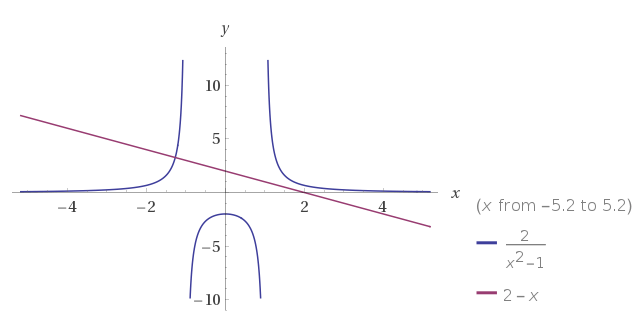
\includegraphics[width=14cm]{rozrahunkova_02/04_01.png}
  \label{fig:rr_02_04_01}
  \centering
\end{figure}

Судячи з графіку, задані лінії мають лише 1 точку пересічення $(\dfrac{2}{x^2-1} = 2-x)$, тому будемо вважати що таку площу знайти неможливо, оскільки вона нічим не обмежена.
 \\ \qquad \\
  {\task{green}{В4 - РР1 - 04.02}} {\descr{Дослідити функцію на неперервність}}

$$
y=3^{\dfrac{2x}{3x+1}}
$$

Дослідимо функцію в точкі $-\dfrac{1}{3}$ де вона можливо має точку розриву.


$$
  \lim_{x \to -1/3 -0} 3^{\dfrac{2x}{3x+1}} \qquad \lim_{x \to (-1/3-0.001) -0} 3^{\dfrac{2x}{3x+1}} = \infty
$$

$$
  \lim_{x \to -1/3 +0} 3^{\dfrac{2x}{3x+1}} \qquad \lim_{x \to (-1/3+0.001) +0} 3^{\dfrac{2x}{3x+1}} = \infty
$$

\textbf{Висновок} - функція в точкі $-\dfrac{1}{3}$ тосить характер розриву \textbf{другого роду}, оскільки границі функції зліва та зправа прямують у нескінченність.


\begin{figure}[h!]
  \centering
  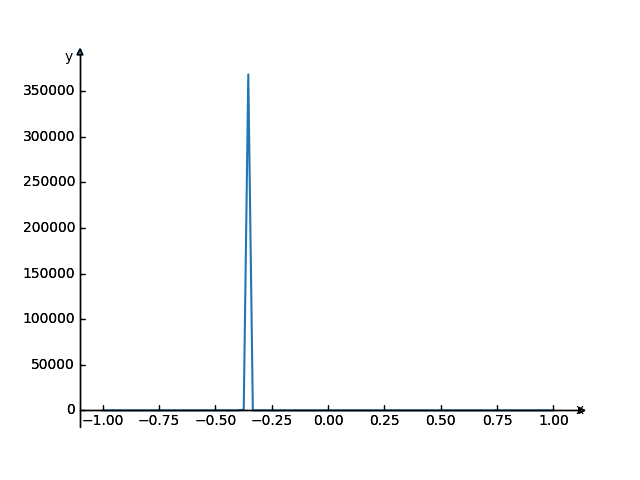
\includegraphics[width=14cm]{rozrahunkova_01/04_02.png}
  \caption{Графік функції}
  \label{fig:rr_01_40_02}
  \centering
\end{figure}
 \\ \qquad \\
  {\task{green}{В4 - РР1 - 05.01}} {\descr[1]{Обчислити площу поверхні, одержаної при обертанні даннної кривої насколо осі OX}}

$$
  y = -\dfrac{1}{2}\ln{x}+\dfrac{x^2}{4} {\qquad} x \in [1;e]
$$

Для знаходження поверхні обертання використаємо наступну формулу

$$Q = 2\pi\int^b_a f(x) \sqrt{1+(f'(x))^2} \d{x} $$

$$
  2\pi \int^e_1 (-\dfrac{1}{2}\ln{x}+\dfrac{x^2}{4}) \sqrt{1+((\dfrac{x^2}{4}-\dfrac{1}{2}\ln{x})')^2} \d{x}
= 2\pi \int^e_1 \dfrac{1}{2} ( \dfrac{x^2}{2} - \ln{x} ) \sqrt{1+(\dfrac{x^2-1}{2x})^2} \d{x}
$$

$$
= \dfrac{2\pi}{2} ( \int^e_1  ( \dfrac{x^2}{2} - \ln{x} ) \sqrt{1+(\dfrac{x^2-1}{2x})^2} \d{x} )
= \pi \int^e_1  \dfrac{x^2}{2} \sqrt{1+(\dfrac{x^2-1}{2x})^2} \d{x} - \pi \int^e_1 \ln{x} \sqrt{1+(\dfrac{x^2-1}{2x})^2}
$$

$$
= \dfrac{\pi}{2} \int^e_1  x^2 \sqrt{\dfrac{4x^2+x^4-2x^2+1}{4x^2}} \d{x} - \pi \int^e_1 \ln{x} \sqrt{\dfrac{4x^2+x^4-2x^2+1}{4x^2}}\d{x}
$$

$$
= \dfrac{\pi}{2} \int^e_1  \dfrac{x^2}{2x} \sqrt{x^4+2x^2+1} \d{x} - \pi \int^e_1 \ln{x} \sqrt{\dfrac{x^2(x^2+2+\dfrac{1}{x^2})}{4x^2}}\d{x}
$$

$$
= \dfrac{\pi}{4} \int^e_1  x  \sqrt{(x^2+1)^2} \d{x} - \pi  \int^e_1 \dfrac{\ln{x}}{2} \sqrt{\dfrac{x^4+2x^2+1}{x^2}}\d{x}
$$

$$
= \dfrac{\pi}{4} \int^e_1  (x^3+x) \d{x} - \dfrac{\pi}{2}  \int^e_1 \ln{x} \sqrt{\dfrac{(x^2+1)^2}{x^2}}\d{x}
$$

$$
= \dfrac{\pi}{4} \int^e_1 x^3\d{x} + \dfrac{\pi}{4} \int^e_1 x \d{x} - \dfrac{\pi}{2}  \int^e_1  \dfrac{(x^2+1)\ln{x}}{x} \d{x}
$$

$$
= \dfrac{\pi}{4} \int^e_1 x^3\d{x} + \dfrac{\pi}{4} \int^e_1 x \d{x} - \dfrac{\pi}{2}( \int^e_1  \dfrac{x^2 \ln{x}}{x} \d{x} + \int^e_1 \dfrac{\ln{x}}{x} \d{x} )
$$


$$
= \dfrac{\pi}{4} \int^e_1 x^3\d{x} + \dfrac{\pi}{4} \int^e_1 x \d{x} - \dfrac{\pi}{2}\Bigg( \int^e_1  x\ln{x} \d{x} + \int^e_1 \dfrac{\ln{x}}{x} \d{x}
  \Bigg|
    \begin{array}{rlrlrlrl}
      u = & \ln{x} & x_1 = & e & y_1 = \ln{e} & = 1 \\
      u'= & \dfrac{1}{x} & x_0 = & 1 & y_0 = \ln{1} & = 0\\
      \end{array}
  \Bigg|
\Bigg)
$$

$$
= \dfrac{\pi}{4} \int^e_1 x^3\d{x} + \dfrac{\pi}{4} \int^e_1 x \d{x} - \dfrac{\pi}{2}( \int^e_1  x\ln{x} \d{x} + \int^1_0 u \d{u} )
$$

$$
= \dfrac{\pi}{4} \int^e_1 x^3\d{x} + \dfrac{\pi}{4} \int^e_1 x \d{x} - \dfrac{\pi}{2} \int^1_0 u \d{u}
 -  \dfrac{\pi}{2}\int^e_1  x\ln{x}  \d{x} \Bigg|
  \begin{array}{rlrl}
      u  =& \ln{x} & v  = & x^2/2 \\
      u' =& 1/x    & v' = & x \\
    \end{array}
\Bigg|
$$

$$
= \dfrac{\pi}{4} \int^e_1 x^3\d{x} + \dfrac{\pi}{4} \int^e_1 x \d{x} - \dfrac{\pi}{2} \int^1_0 u \d{u} -  \dfrac{\pi}{2} (\dfrac{x^2\ln{x}}{2} \Bigg|^e_1 - \int^e_1 \dfrac{1}{x} \dfrac{x^2}{2} \d{x} )
$$

$$
= \dfrac{\pi}{4} \int^e_1 x^3\d{x} + \dfrac{\pi}{4} \int^e_1 x \d{x} - \dfrac{\pi}{2} \int^1_0 u \d{u} -  \dfrac{\pi}{2} (\dfrac{x^2\ln{x}}{2} \Bigg|^e_1 - \dfrac{1}{2}\int^e_1 x\d{x} )
$$

Для більшої зручності порведемо обчислення визначених інтегралів окремо (формула вже завелика для копіювання навіть при наборі в LaTeX).

$$
1) \dfrac{\pi}{4} \int^e_1 x^3\d{x}
  = \dfrac{\pi}{4} \times \dfrac{x^4}{4}  \Bigg|^e_1
  = \dfrac{\pi}{16} (x^4) \Bigg|^e_1
  = \dfrac{\pi}{16} (e^4- 1^4)
  = \dfrac{\pi}{16} (e^4- 1)
$$

$$
2) \dfrac{\pi}{4} \int^e_1 x \d{x}
= \dfrac{\pi}{4} \times \dfrac{x^2}{2}  \Bigg|^e_1
= \dfrac{\pi}{8} (x^2) \Bigg|^e_1
= \dfrac{\pi}{8} (e^2 - 1^2)
= \dfrac{\pi}{8} (e^2 - 1)
$$


$$
3) - \dfrac{\pi}{2} \int^1_0 u \d{u} = - \dfrac{\pi}{4} (u^2)\Bigg|^1_0 = - \dfrac{\pi}{4} (1^2-0^2) = -\dfrac{\pi}{4}
$$

$$
4)  -  \dfrac{\pi}{2} \times \dfrac{x^2\ln{x}}{2} \Bigg|^e_1
= - \dfrac{\pi}{4} (e^2\ln{e}-1^2\ln{1})
= - \dfrac{\pi}{4} (e^2 \times 1 - 1^2 \times 0}) =
= - \dfrac{\pi e^2}{4}
$$

$$
5) - \dfrac{\pi}{2} \times -\dfrac{1}{2} \int^e_1 x\d{x}
= \dfrac{\pi}{4} \times \dfrac{x^2}{2}  \Bigg|^e_1
= \dfrac{\pi}{8} \times ( x^2 ) \Bigg|^e_1
= \dfrac{\pi}{8} \times ( e^2 - 1^2)
= \dfrac{\pi}{8} \times ( e^2 - 1)
$$

Залишилось лише просумувати отримані площі.

$$
\dfrac{\pi}{16} (e^4- 1) + \dfrac{\pi}{8} (e^2 - 1) -\dfrac{\pi}{4} - \dfrac{\pi e^2}{4} + \dfrac{\pi}{8} \times ( e^2 - 1)
= \dfrac{\pi}{16} (e^4- 1) + \dfrac{\pi}{4} (e^2 - 1) -\dfrac{\pi}{4} - \dfrac{\pi e^2}{4}
$$

$$
= \dfrac{\pi( (e^4-1) + 4(e^2-1) - 4 -4e^2)}{16}
= \dfrac{\pi( e^4-1 + 4e^2-4 - 4 -4e^2)}{16}
= \dfrac{\pi( e^4-9 ) }{16}
$$


$$
\boxed{ Q = \dfrac{\pi( e^4-9 ) }{16} }
$$
 \\ \qquad \\
  {\task{green}{В4 - РР1 - 05.02}} {\descr{Знайти похідну функції:}}

$$
  y = \sqrt{x^3+2x+\dfrac{1}{x}} = (x^3+2x+\dfrac{1}{x})^{\dfrac{1}{2}}
$$

$$
  y' = ((x^3+2x+\dfrac{1}{x})^{\dfrac{1}{2}})'
     =  \dfrac{1}{2}(x^3+2x+\dfrac{1}{x})^{-\dfrac{1}{2}}(x^3+2x+\dfrac{1}{x})'
     =  \dfrac{1}{2}(x^3+2x+\dfrac{1}{x})^{-\dfrac{1}{2}}(3x^2+2+\dfrac{1}{x^2})
$$

$$
  y' = \dfrac{3x^2+2+\dfrac{1}{x^2}}{2\sqrt(x^3+2x+\dfrac{1}{x})}
$$
 \\ \qquad \\
  {\task{green}{В4 - РР1 - 05.03}} {\descr{Знайти похідну функції:}}

$$
  y = \dfrac{\arccos\sqrt{x}}{x}
$$
$$
  y' = \dfrac{(\arccos\sqrt{x})'(x)-(\arccos\sqrt{x})(x)'}{x^2}
     = \dfrac{-\dfrac{x}{\sqrt{1-(\sqrt{x})^2}}(\sqrt{x})'-\arccos\sqrt{x}}{x^2} =
$$
$$
    = \dfrac{-\dfrac{x}{\sqrt{1-x}}\cdot\dfrac{1}{2\sqrt(x)}-\arccos\sqrt{x}}{x^2}
     = - \dfrac{\dfrac{x}{2\sqrt{x}\sqrt{1-x}}+\arccos\sqrt{x}}{x^2}.
$$
 \\ \qquad \\
  {\task{green}{В4 - РР1 - 05.04}} {\descr{Знайти похідну функції:}}

$$
  \begin{array}{r c l}
    y  & = & (x^3-x^2)^x \\
    y' & = & ((x^3-x^2)^x)' \\
    (\ln y)' & = & (\ln(x^3-x^2)^x)' \\
    \\
    \dfrac{1}{y}y' & = & x \dfrac{1}{x^3-x^2}(x^3-x^2)' \\
  \end{array}
$$

$$
  y' = x(x^3-x^2)^x \dfrac{1}{x^3-x^2}(3x^2-2x)
      = \dfrac{x (x^3-x^2)^x(3x^2-2x)}{x^3-x^2}
$$
$$
  y' = (x^3-x^2)^{x-1}(3x^3-2x^2).
$$

% \begin{array}{r c l}
%   \dfrac{1}{y}y' & = & x \dfrac{1}{x^3-x^2}(x^3-x^2)' \\
%   \dfrac{y'}{y}  & = & x \dfrac{1}{x^3-x^2}(3x^2-2x) \\
%   y' & = & x (x^3-x^2)^x \dfrac{1}{x^3-x^2}(3x^2-2x) \\
%   y' & = & \dfrac{x (x^3-x^2)^x(3x^2-2x)}{x^3-x^2} \\
%   \\
%   y' & = & \dfrac{(x^3-x^2)^x(3x^3-2x^2)}{x^3-x^2} \\
%   \\
%   y' & = & (3x^3-2x^2)(x^3-x^2)^{x-1} \\
%   \end{array}
 \\ \qquad \\
  {\task{green}{В4 - РР1 - 05.05}} {\descr{Знайти похідну функції:}}

$$
 y = 5^{\tg^2{x}}
$$

$$
y' = (5^{\tg^2{x}})' = 5^{\tg^2{x}} \cdot \ln{5} \cdot ((\tg{x})^2)' = 5^{\tg^2{x}} \cdot \ln{5} \cdot 2 \tg{x} \cdot \dfrac{1}{\cos^2{x}}
$$
 \\ \qquad \\
  {\task{green}{В4 - РР1 - 05.06}} {\descr{Знайти похідну функції:}}

$$
x\tg{y}-y{\tg{x}} = 2
$$

$$
x\tg{y}-y{\tg{x}} - 2 = 0
$$

$$
 0 = (x\tg{y})'-(y{\tg{x}})' - (2)' = ( (x)'\tg{y} + x(\tg{y})' ) - ((y)'\tg{x} + y(\tg{x})') = (x'\tg{y} + \dfrac{x}{\cos^2{y}}) - (y'\tg{x}+\dfrac{y}{\cos^2{x}})
$$

$$
y'\tg{x}+\dfrac{y}{\cos^2{x}} = x'\tg{y} + \dfrac{x}{\cos^2{y}}
$$

$$
y'\tg{x}
  = x'\tg{y} + \dfrac{x}{\cos^2{y}} - \dfrac{y}{\cos^2{x}}
$$

$$
  y' = \dfrac{\tg{y}}{\tg{x}}   + \dfrac{x}{\tg{x}\cos^2{y}}   - \dfrac{y}{\tg{x}\cos^2{x}}
$$
 \\ \qquad \\
  {\task{green}{В4 - РР1 - 05.07}} {\descr{Знайти похідну функції:}}

\begin{displaymath}
  \left\{\begin{array}{rl}
    x =& \dfrac{1}{t+2} \\
    y =& \dfrac{t^2}{(t+2)^2}
  \end{array} \qquad y'_x=? \qquad y''_xx=?
\end{displaymath}

$$
  y'_x=\dfrac{y'}{x'} \qquad y''_xx=\dfrac{y'_x}{x'}
$$

$$
  x' = \Big(\dfrac{1}{t+2}\Big)' = \dfrac{1}{(t+2)^2}(t+2)' = \dfrac{1}{(t+2)^2}
$$

$$
  y' = \Big(\dfrac{t^2}{(t+2)^2}\Big)'
     = \dfrac{(t^2)'(t+2)^2-(t^2)((t+2)^2)'}{(t+2)^4}
     = \dfrac{2t(t+2)^2-2t^2(t+2)}{(t+2)^4}
     = \dfrac{(2t(t+2)-2t^2)(t+2)}{(t+2)^4}
$$
$$
  y' = \dfrac{2t(t+2)-2t^2}{(t+2)^3} = \dfrac{2t((t+2)-t)}{(t+2)^3}= \dfrac{4t}{(t+2)^3}
$$

$$
  y'_{x}
    = \dfrac{y'}{x'}
    = \dfrac{\dfrac{4t}{(t+2)^3}}{\dfrac{1}{(t+2)^2}}
    = \dfrac{4t(t+2)^2}{(t+2)^3}
    = \dfrac{4t}{t+2}
$$

$$
  y''_{xx} = \dfrac{(y'_{x})'}{x'}
    = \dfrac{\Big(\dfrac{4t}{t+2}\Big)'}{\dfrac{1}{(t+2)^2}}
    = (t+2)^2 \dfrac{(4t)'(t+2)-(4t)(t+2)'}{(t+2)^2}
    = \dfrac{(4t+8-4t)(t+2)^2}{(t+2)^2} = 8
$$
 \\ \qquad \\

  {\task{green}{В4 - РР1 - 06.01}} {\descr[1]{Знайти обєм тіла, одержаного прі обертанні криволінійного заданого сектора навколо полярної осі:}}

$$
\rho = \alpha \sqrt{\cos{\varphi}},{\qquad} \varphi \in \Big[ 0; \dfrac{\pi}{2} \Big]
$$

Об'єм  тіла  отирманого обертанням в навколо полярної осі заданого двума поялрними координатами можна знайти за формулою
$$
V = \dfrac{2\pi}{3} \int_{\alpha}^{\beta} \rho^3\sin{\varphi} \d{\varphi}
$$

% http://energy.bmstu.ru/gormath/mathan2s/usint/UsingInt.htm#s121
$$
\dfrac{2\pi}{3} \int_0^{\dfrac{\pi}{2}} (a\sqrt{\cos{\varphi}})^3\sin{\varphi} \d{\varphi}
= \dfrac{2\pi}{3} \int_0^{\dfrac{\pi}{2}} a^3 \cos{\varphi}^{\dfrac{3}{2}}  \sin{\varphi} \d{\varphi}
\Bigg|
  \begin{array}{rl rl r}
     u =& \sin{\varphi} & \varphi_2 = & \dfrac{\pi}{2} & u_2 =   1  \\
    \d{u} =& \cos{\varphi} & \varphi_1 = & 0 & u_1 =   0 \\
  \end{array}
\Bigg| = \dfrac{2\pi a^4 }{3} \int^1_0 u^{\dfrac{3}{2}}\d{u}
$$

$$
= \dfrac{2\pi a^4 }{3} \int^1_0 u^{\dfrac{3}{2}}\d{u}
= \dfrac{a^4 \pi}{6} \dfrac{u^{\dfrac{5}{2}}}{\dfrac{5}{2}} \Bigg|_0^{1}
= \dfrac{a^4 \pi}{15} \sqrt{u^5} \Bigg|_0^{1}
= \dfrac{a^4 \pi}{15}
$$

$$
\boxed{V = \dfrac{a^4 \pi}{15} }
$$
 \\ \qquad \\
  {\task{green}{В4 - РР1 - 07.01}} {\descr{Провести повне дослідження функції і побудувати графік}}

$$
y=\dfrac{2}{x^2+2x}
$$


1) $x \in (-\infty;-2)\cup(-2;0)\cup(0;+\infty)$

2) Графік не перетинає ось $x$.

3) Функція непарна оскільки

$$
  f(-x) = \dfrac{2}{(-x)^2+2(-x)} = \dfrac{2}{x^2-2x}
$$

4) Обидві точки -2 та 0 носить характер розриву другого роду оскільки вони прямують в безмежність.

$$
  \lim_{x \to -2 \ \pm0} \dfrac{2}{x^2+2x} = \mp \infty \qquad   \lim_{x \to 0 \ \pm0} \dfrac{2}{x^2+2x} = \pm \infty
$$

5) Похідна
$$
  y' = (\dfrac{2}{x^2+2x})'
     = \dfrac{2'(x^2+2x)-2(x^2+2x)'}{(x^2+2x)^2}
     = \dfrac{-4x-4}{(x^2+2x)^2}
$$

Функція не існує в точках $x=-2$ та $x=0$, а $x=-1$ є критичною (такою що є підозрілою на екстремум мінімум або максимум). На інтервалі $(-\infty;+\infty)$ матимемо:



\begin{center}
  \begin{tabular}{ | c | c | c | c | c | c | c | c | }
    \hline
      x     & (-\infty;-2) & -2 & (-2;-1) & -1 & (-1:0) & 0 &  (0; +\infty) \\
      \hline
      f'(x) &  + & не існує & + & 0  & -  & не існує & - \\
      \hline
      f(x)  & \nearrow  & не існує & \nearrow  & y_{max} = -2  & \searrow   & не існує & \searrow \\
    \hline
  \end{tabular}
\end{center}



6) Друга похідна

$$
  y'' = (\dfrac{-4x-4}{(x^2+2x)^2})'
  = \dfrac{(-4x-4)'(x^2+2x)^2 - (-4x-4)((x^2+2x)^2)' }{(x^2+2x)^4}
$$

$$
= \dfrac{-4(x^2+2x) + 4(2x+2)^2 }{(x^2+2x)^3}
= \dfrac{-4x^2-8x + 16x^2+32x+16 }{(x^2+2x)^3}
= \dfrac{12x^2+24x+16 }{(x^2+2x)^3}
$$

\begin{center}
  \begin{tabular}{ | c | c | c | c | c | c |  }
    \hline
    x & (-\infty;-2) & -2 & (-2:0) & 0 & (0:+\infty) \\
    \hline
    f"(x) &  + & не існує  & - & не існує & +  \\
    \hline
    f(x) &  \cup & не існує  & \cap & не існує & \cup \\
    \hline
  \end{tabular}
\end{center}

7) з пункта (4) випливає що фунція має вертикальні асимптоти в точках $x=-2$ та $x=0$.

Знаходимо горизонтальні асимптоти за формулами (через границі функції):
$$
  y = kx+b
$$

$$
  k = \lim_{x\to\infty} \dfrac{y(x)}{x}
    = \lim_{x\to\infty} \dfrac{2}{x(x^2+2x)}
    = \lim_{x\to\infty} \dfrac{2/x^2}{x(1+2/x)}
    = \dfrac{1}{\infty}
    = 0
$$

$$
  b = \lim_{x\to\infty} (y(x) - kx)
    = \lim_{x\to\infty} \dfrac{2}{x^2+2x}
    = \lim_{x\to\infty} \dfrac{2/x^2}{1+2/x}
    = \dfrac{0}{1}
    = 0
$$

8) Враховуючи висновки ослідження функції будуємо графік:

\begin{figure}[h!]
  \centering
  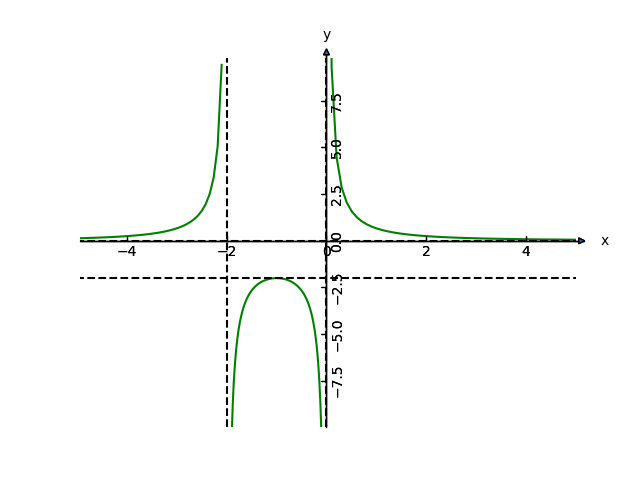
\includegraphics[width=14cm]{rozrahunkova_01/07_01.png}
  \caption{Графік функції $y=\dfrac{2}{x^2+2x}$ }
  \label{fig:rr_01_07_01}
  \centering
\end{figure}
 \\ \qquad \\
  {\task{gray}{В4 - РР1 - 07.02}} {\descr{Провести повне дослідження функції і побудувати графік}}

$$
\rho =\alpha (1-cos2\varphi)
$$
 \\ \qquad \\



\end{document}
